\documentclass{standalone}

\usepackage{listings}
\usepackage{tikz}
\usetikzlibrary{positioning,fit,calc}

\begin{document}
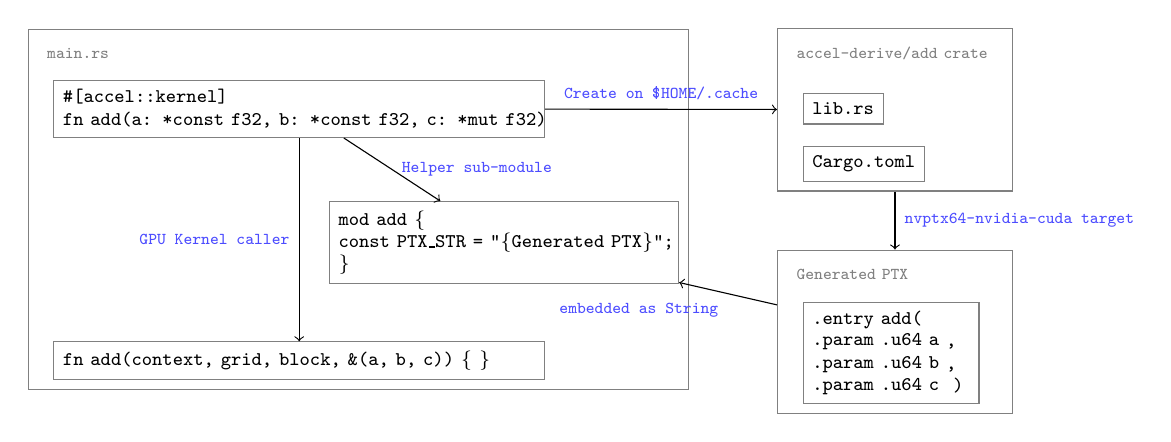
\begin{tikzpicture}[
  node distance=7mm,
  title/.style={font=\fontsize{6}{6}\color{black!50}\ttfamily},
  typetag/.style={rectangle, draw=black!50, font=\scriptsize\ttfamily, anchor=west},
  arrow-annotate/.style={midway, font=\fontsize{6}{6}\color{blue!70}\ttfamily}
]
  \node (main) [title] {main.rs};
  \node (proc-macro) [below=of main.west, typetag, xshift=2mm, text width=6cm] {
    \#[accel::kernel]
    \parbox{8cm}{fn add(a: *const f32, b: *const f32, c: *mut f32)}
  };
  \node (main-ptx) [below=of proc-macro.west, xshift=35mm, yshift=-1cm, typetag, text width=42mm] {
      mod add \{
        \parbox{5cm}{const PTX\_STR = "\{Generated PTX\}";}
      \}
  };
  \node (main-caller) [below=of proc-macro.west, yshift=-25mm, typetag, text width=6cm] {
      fn add(context, grid, block, \&(a, b, c)) \{ \}
  };
  \draw[->] (proc-macro) -- (main-ptx) node[arrow-annotate, right] {Helper sub-module};
  \draw[->] (proc-macro) -- (main-caller) node[arrow-annotate, left] {GPU Kernel caller};
  \node[draw=black!50, fit={(main) (proc-macro) (main-ptx) (main-caller)}] {};

  \node (ptx-builder-title) at (9cm, 0) [title, right, text width=25mm] {accel-derive/add crate};
  \node (lib)  [below=of ptx-builder-title.west, typetag, xshift=2mm] {lib.rs};
  \node (toml) [below=of lib.west, typetag] {Cargo.toml};
  \node (ptx-builder) [draw=black!50, fit={(ptx-builder-title) (lib) (toml)}] {};

  \draw[->] (proc-macro) -- (ptx-builder) node[arrow-annotate, above] {Create on \$HOME/.cache};

  \node (ptx-title) at (9cm, -28mm) [title, right, text width=25mm] {Generated PTX};
  \node (ptx-add)  [below=of ptx-title.west, typetag, xshift=2mm, yshift=-3mm, text width=2cm] {
    .entry add(
    \parbox{17mm}{.param .u64 a},
    \parbox{17mm}{.param .u64 b},
    \parbox{17mm}{.param .u64 c}
    )
  };
  \node (ptx) [draw=black!50, fit={(ptx-title) (ptx-add)}] {};

  \draw[->] (ptx-builder) -- (ptx) node[arrow-annotate, right] {nvptx64-nvidia-cuda target};
  \draw[->] (ptx) -- (main-ptx) node[arrow-annotate, below left]{embedded as String};

\end{tikzpicture}
\end{document}
